
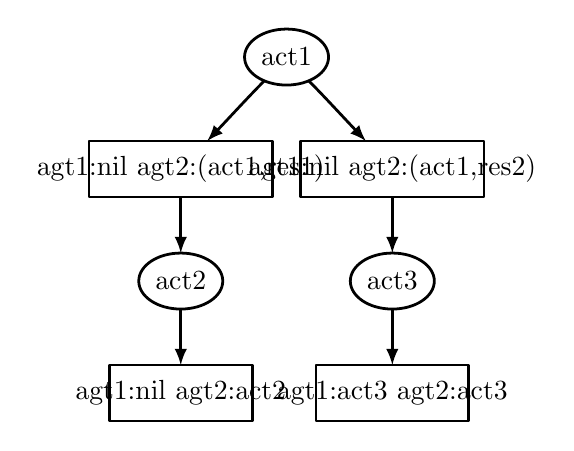
\begin{tikzpicture}[>=latex,join=bevel,scale=0.56]
  \pgfsetlinewidth{1bp}
%
\pgfsetcolor{black}
  % Edge: n1 -> n2
  \draw [->] (113bp,219bp) .. controls (104bp,210bp) and (93bp,198bp)  .. (76bp,180bp);
  % Edge: n1 -> n3
  \draw [->] (141bp,219bp) .. controls (150bp,210bp) and (161bp,198bp)  .. (178bp,180bp);
  % Edge: n4 -> n5
  \draw [->] (59bp,72bp) .. controls (59bp,64bp) and (59bp,55bp)  .. (59bp,36bp);
  % Edge: n6 -> n7
  \draw [->] (195bp,72bp) .. controls (195bp,64bp) and (195bp,55bp)  .. (195bp,36bp);
  % Edge: n2 -> n4
  \draw [->] (59bp,144bp) .. controls (59bp,136bp) and (59bp,127bp)  .. (59bp,108bp);
  % Edge: n3 -> n6
  \draw [->] (195bp,144bp) .. controls (195bp,136bp) and (195bp,127bp)  .. (195bp,108bp);
  % Node: n1
\begin{scope}
  \pgfsetstrokecolor{black}
  \draw (127bp,234bp) ellipse (27bp and 18bp);
  \draw (127bp,234bp) node {act1};
\end{scope}
  % Node: n2
\begin{scope}
  \pgfsetstrokecolor{black}
  \draw (118bp,180bp) -- (0bp,180bp) -- (0bp,144bp) -- (118bp,144bp) -- cycle;
  \draw (59bp,162bp) node {agt1:nil agt2:(act1,res1)};
\end{scope}
  % Node: n3
\begin{scope}
  \pgfsetstrokecolor{black}
  \draw (254bp,180bp) -- (136bp,180bp) -- (136bp,144bp) -- (254bp,144bp) -- cycle;
  \draw (195bp,162bp) node {agt1:nil agt2:(act1,res2)};
\end{scope}
  % Node: n4
\begin{scope}
  \pgfsetstrokecolor{black}
  \draw (59bp,90bp) ellipse (27bp and 18bp);
  \draw (59bp,90bp) node {act2};
\end{scope}
  % Node: n5
\begin{scope}
  \pgfsetstrokecolor{black}
  \draw (105bp,36bp) -- (13bp,36bp) -- (13bp,0bp) -- (105bp,0bp) -- cycle;
  \draw (59bp,18bp) node {agt1:nil agt2:act2};
\end{scope}
  % Node: n6
\begin{scope}
  \pgfsetstrokecolor{black}
  \draw (195bp,90bp) ellipse (27bp and 18bp);
  \draw (195bp,90bp) node {act3};
\end{scope}
  % Node: n7
\begin{scope}
  \pgfsetstrokecolor{black}
  \draw (244bp,36bp) -- (146bp,36bp) -- (146bp,0bp) -- (244bp,0bp) -- cycle;
  \draw (195bp,18bp) node {agt1:act3 agt2:act3};
\end{scope}
%
\end{tikzpicture}

